\begin{figure}[ht]
\begin{minipage}{.49\textwidth}
    \centering
    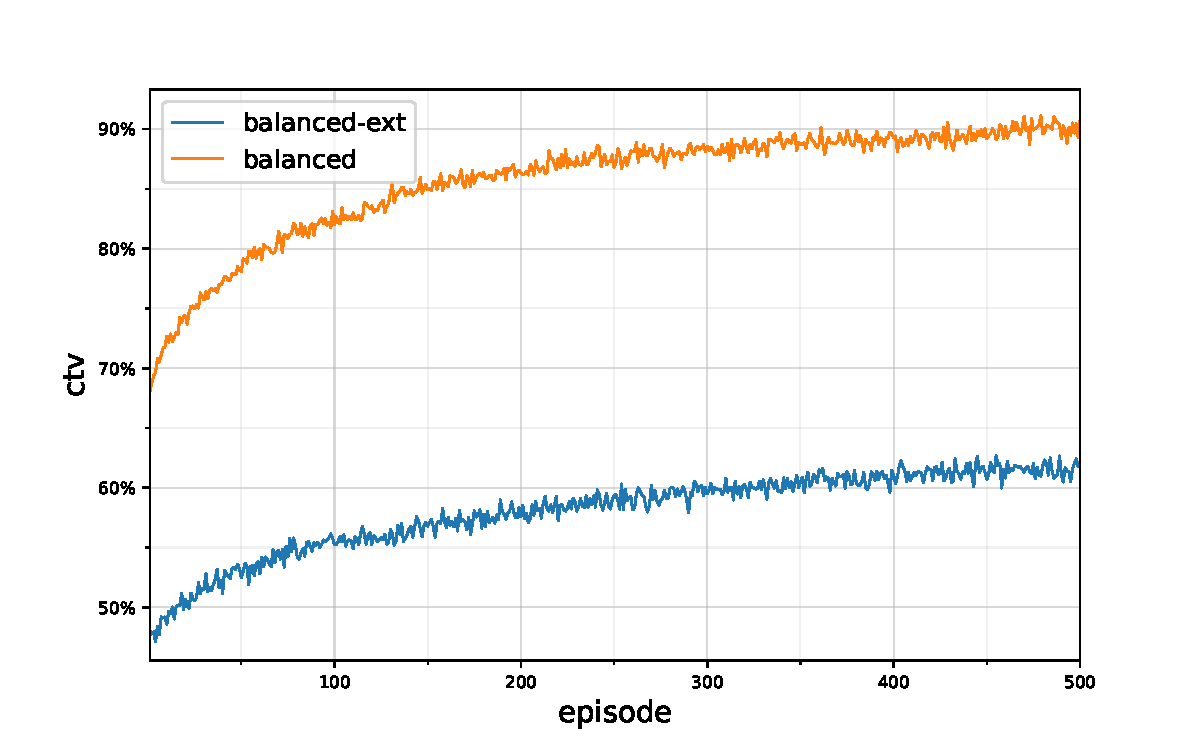
\includegraphics[width=1.0\linewidth,trim={25pt 0pt 50pt 0pt},clip]{5balanced_ctv-optimal-ctv}
    \captionsetup{labelfont=bf,singlelinecheck=on}
    \caption{System utility compared to the theoretical \newline maximum for the \simulationSimple{}{} system.}
    \label{fig:5_ctvoptimalctv}
\end{minipage}\hfill% 
\begin{minipage}{.49\textwidth}
	\centering
	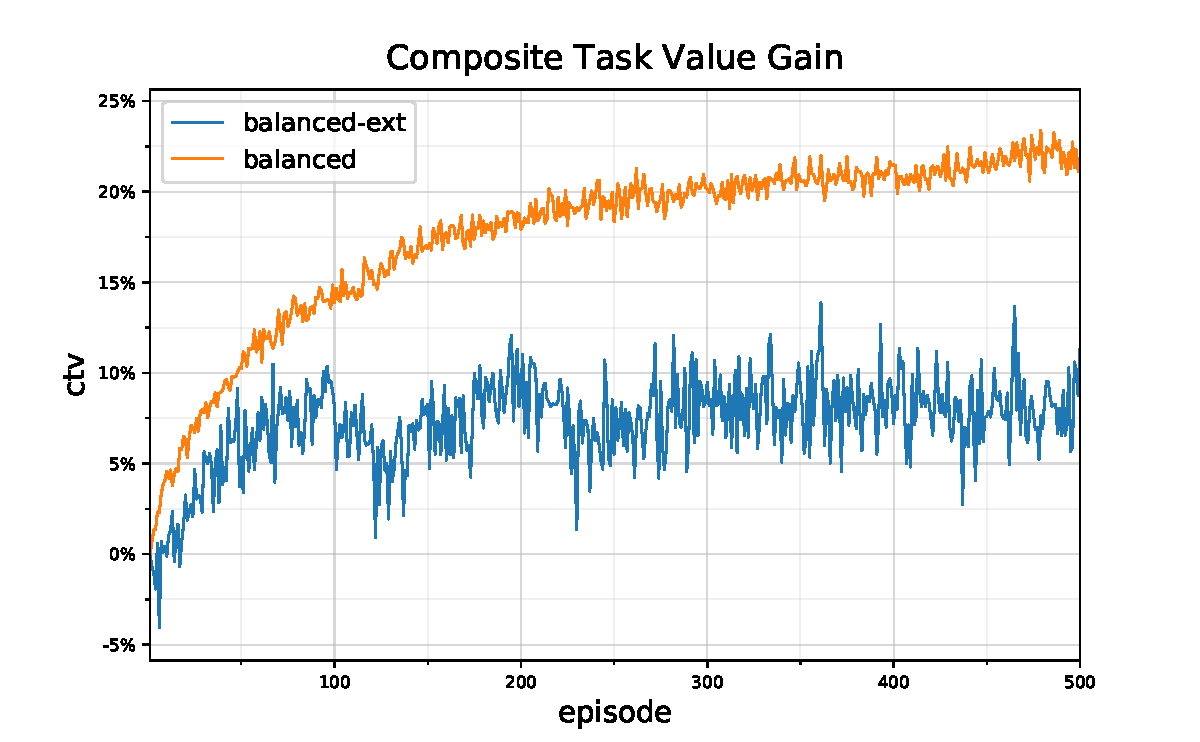
\includegraphics[width=1.0\linewidth,trim={25pt 0pt 50pt 0pt},clip]{5balanced_ctv-optimal-ctv-gain}
	\captionsetup{labelfont=bf,singlelinecheck=on}
	\caption{System utility percentage increase over each \newline systems' lifetime.}
	\label{fig:5_ctv-optimal-ctv-gain}
\end{minipage}
\end{figure}
\begin{figure}[ht]
	\begin{minipage}{.49\textwidth}
		\centering
		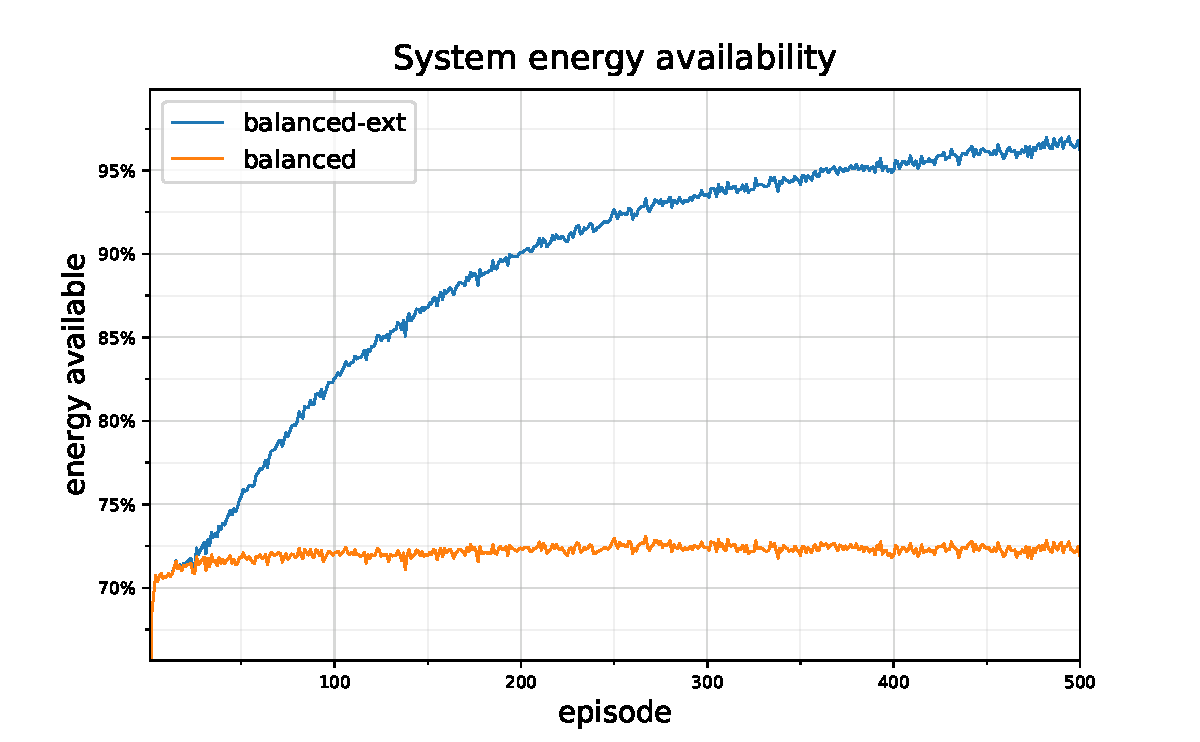
\includegraphics[width=1.0\linewidth,trim={25pt 0pt 50pt 0pt},clip]{5balanced_ctv-statistics-energy-available}
		\captionsetup{labelfont=bf,singlelinecheck=on}
		\caption{Energy available in the \simulationSimple{}{} and \simulationExtended{}{} \newline systems as percentage of the maximum possible.}
		\label{fig:ctv-statistics-energy-available}
	\end{minipage}\hfill% 
	\begin{minipage}{.49\textwidth}
		\centering
		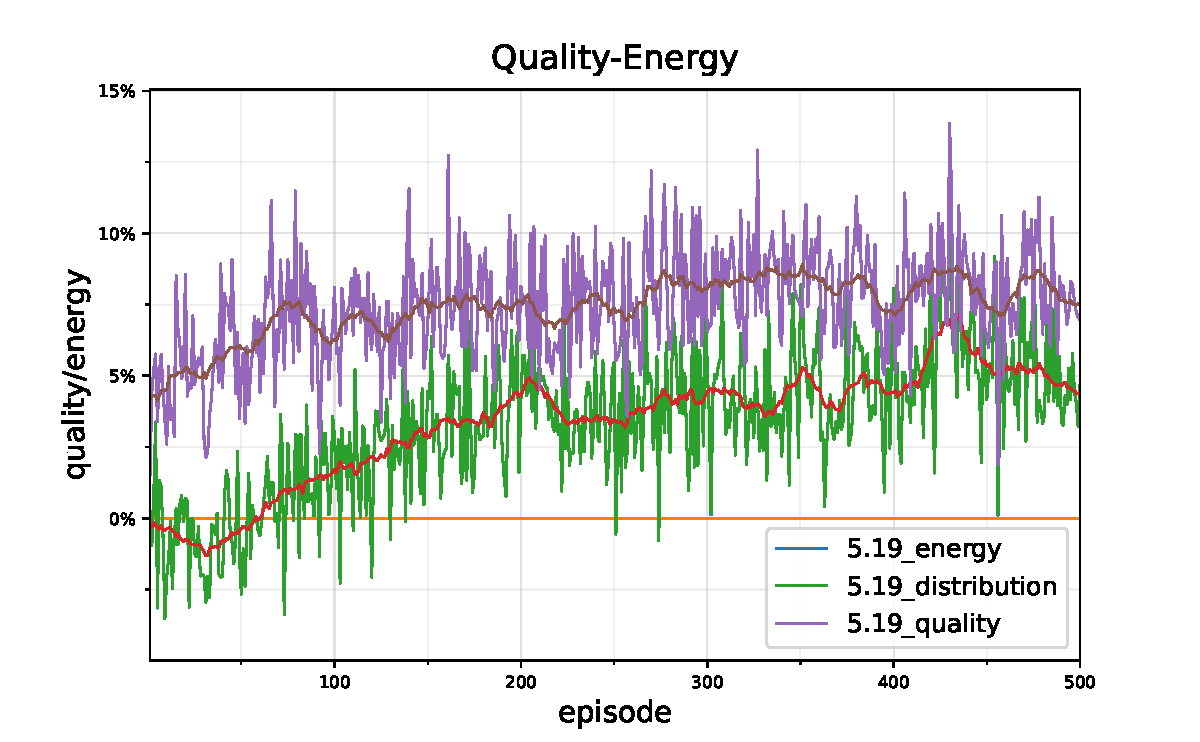
\includegraphics[width=1.0\linewidth,trim={25pt 0pt 50pt 0pt},clip]{5.19_ctv-quality-energy-baseline-comparison}
		\caption{Task quality to energy available ratio in the \newline  \simulationExtended{}{} system, with \algorithmEnergy{}{} as the baseline}
		\label{fig:ctv-quality-energy-baseline-comparison}
	\end{minipage}
\end{figure}
\begin{figure}[ht]
	\begin{minipage}{.49\textwidth}
		\centering
		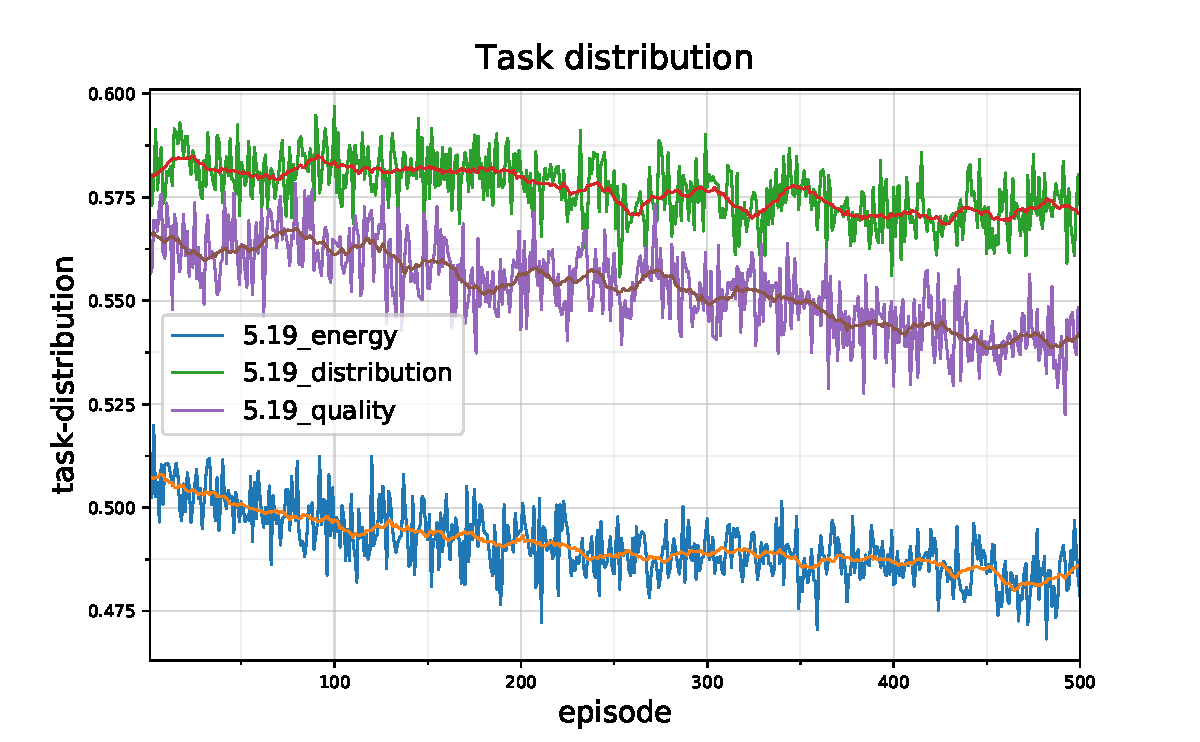
\includegraphics[width=1.0\linewidth,trim={25pt 0pt 50pt 0pt},clip]{5.19_ctv-task-distribution-comparison}
		\caption{Task distribution in the \simulationExtended{}{} \newline system}
		\label{fig:ctv-task-distribution-comparison}
	\end{minipage}\hfill% 
	\begin{minipage}{.49\textwidth}
		\centering
		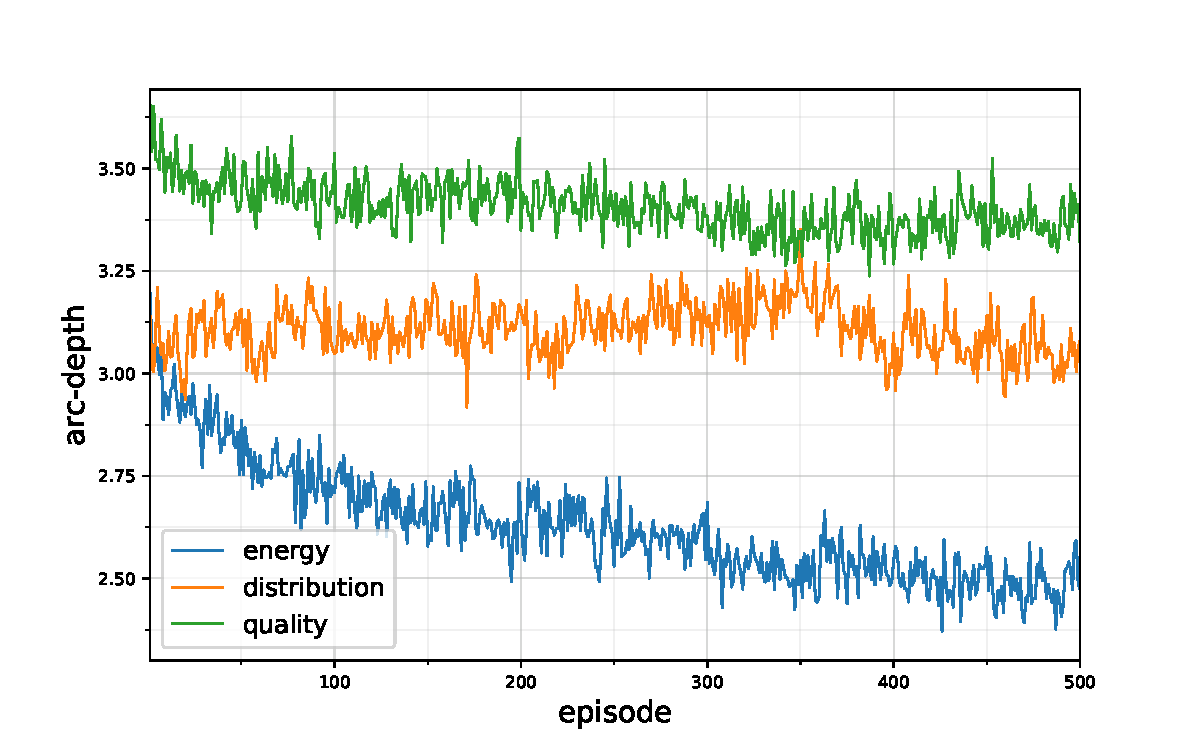
\includegraphics[width=1.0\linewidth,trim={25pt 0pt 50pt 0pt},clip]{5.19_ctv-arc-depth-comparison}
		\caption{Comparison of arc-depths in the \simulationExtended{}{} \newline system}
		\label{fig:ctv-arc-depth-comparison}
	\end{minipage}
\end{figure}
As seen in Figure \ref{fig:5_ctv-optimal-ctv-gain}, the \algorithmBalanced{}{} algorithm optimises the utility by \resultsCTVBalancedDiff{}{}  in the \simulationSimple{}{} system and by \resultsCTVBalancedExtDiff{}{} in the \simulationExtended{}{} system over the $500$ episodes. The energy available in the systems overall is shown in Figure \ref{fig:ctv-statistics-energy-available}. As the algorithm improves the routing for task allocation, the energy consumption of the system is reduced, the available energy going from \resultsEnergyBalancedStart{}{} to \resultsEnergyBalancedEnd{}{} in the \simulationSimple{}{} system, and by \resultsEnergyBalancedExtStart{}{} to \resultsEnergyBalancedExtEnd{}{} in the \simulationExtended{}{} one. Note that the task values theoretical maximum becomes less statistically likely to be achievable the larger the system due to the ad-hoc, random layout of the nodes. Importantly however, the task-values themselves are shown to optimised by the algorithm. In contrast, for energy availability, in larger systems there is more possible arc configurations that can complete tasks, and more nodes that are not involved, so the  energy consumption as a fraction of energy overall is reduced. In both the \simulationSimple{}{} and \simulationExtended{}{} systems though, we see the energy availability in the system overall increasing with system time.

We now look at the extended system in detail to examine how the algorithm vary the balance  of optimisation over the CTV components, allowing multiple-objectives to be targeted. Figure 	\ref{fig:ctv-quality-energy-baseline-comparison} shows the task quality to energy availability ratio. 
As quality is preferentially optimised for over energy availability, values range higher. The \algorithmQuality{}{} algorithm, with its higher $\gamma$ value, optimises for task values by \resultsQEQualityEnd{}{} over the \algorithmEnergy{}{} algorithm, and the \algorithmDistribution{}{} algorithm by \resultsQEDistDiff{}{}. The task distribution of the \algorithmDistribution{}{} algorithm, shown in Figure 	\ref{fig:ctv-task-distribution-comparison}, remains relatively steady throughout the system lifetime at \resultsTaskDistDistStart{}{} to \resultsTaskDistDistEnd{}{}, dropping only \resultsTaskDistDistPercent{}{}. The \algorithmQuality{}{} algorithm starts slightly lower than this at \resultsTaskDistQualityStart{}{} and falls \resultsTaskDistQualityPercent{}{} to \resultsTaskDistQualityEnd{}{}. Notably the \algorithmEnergy{}{} algorithm starts and remains at a significantly lower distribution than both these algorithms at \resultsTaskDistEnergyEnd{}{}, dropping \resultsTaskDistEnergydPercent{}{}. Figure
\ref{fig:ctv-arc-depth-comparison} shows the related effect on arc-depths for each algorithm. The \algorithmQuality{}{} and \algorithmDistribution{}{} algorithms have relatively stable arc depths at \resultsArcDepthQualityEnd{}{} and \resultsArcDepthDistEnd{}{} respectively. The average arc-depth of the \algorithmEnergy{}{} algorithm however drops from \resultsArcDepthEnergyStart{}{} to  \resultsArcDepthEnergyEnd{}{} over the systems' lifetime, a \resultsArcDepthEnergyPercent{}{} decrease.

\begin{figure}
	\centering
	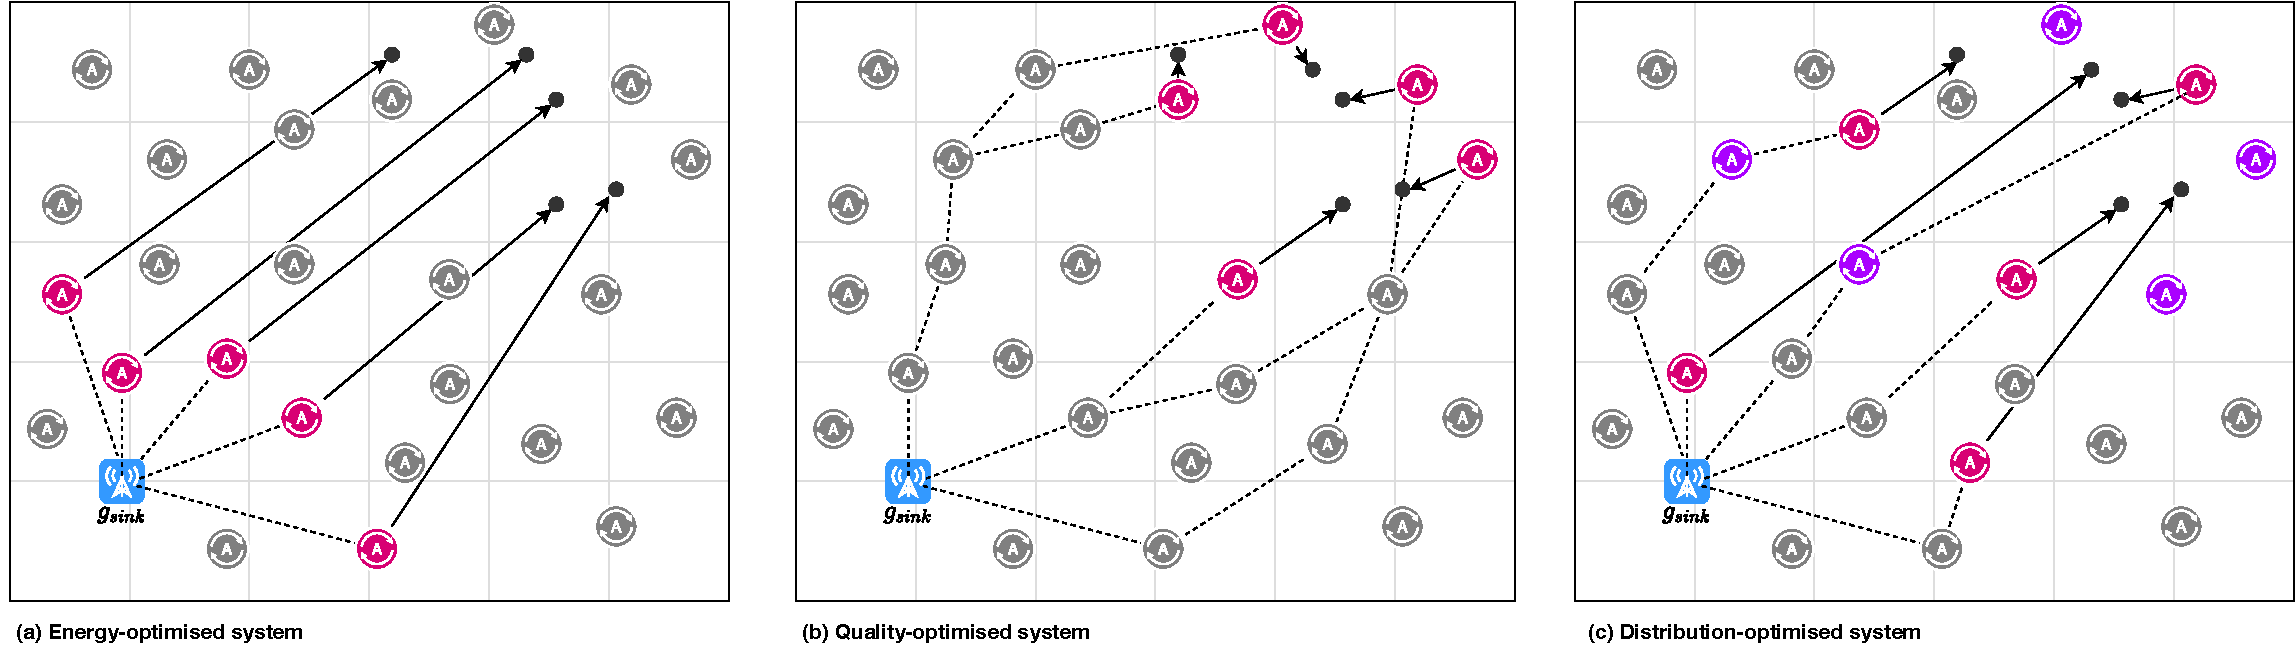
\includegraphics[width=1.0\linewidth]{result-types}
	\caption{Three sample arc patterns in the \simulationExtended{}{} system. In the \algorithmEnergy{}{}-optimised configuration (a), the sensing agents are near the sync agent. Energy use is minimised but the measurements task-values are low. In the \algorithmQuality{}{}-optimised configuration (b) the sensing agents are close to the demand points, maximising the task-values, however there is an increase in energy usage as they are more distant from the sink, with increased arc-length. In the \algorithmDistribution{}{}-optimised configuration (c), sensing agents are a mix of close and further away from the demand points, with an the agents participating in the arcs changing with different measurements}
	\label{fig:result-types}
\end{figure}
Relating these results to the systems in Figure \ref{fig:result-types}, the \algorithmEnergy{}{} algorithm is close to configuration in Figure \ref{fig:result-types}$(a)$, where energy consumption is reduced by using shorter arc-lengths and so, the amount of energy used by agents in the system to broadcast task re-allocations. The cost of this is that the tasks are completed to a lower quality. In Figure \ref{fig:result-types}$(c)$, arc-lengths are large so that tasks can be completed by agents close to their demand points, increasing task quality as well as consumption, as seen in the results for the \algorithmQuality{}{} algorithm. The configuration in Figure \ref{fig:result-types}$(b)$ explains the results seen with the \algorithmDistribution{}{} algorithm, where tasks are completed by an increased number of different agents with different arc-lengths and task qualities, giving a greater distribution of task completions and energy usage, but with more energy consumption overall than the \algorithmEnergy{}{} algorithm, and less task-quality than the \algorithmQuality{}{} algorithm.

As seen both the \simulationSimple{}{} and \simulationExtended{}{} system configurations, utility and energy availability are both optimised by the algorithm, showing it achieves two of the main goals for applications in WSN. Additionally, the results of the \algorithmEnergy{}{}, \algorithmQuality{}{}, and \algorithmDistribution{}{}-optimised algorithms in the \simulationExtended{}{} system show that we can adapt the balance of the CTV components through varying values of $\alpha$, $\beta$, and $\gamma$, to achieve an adaptive multi-objective optimisation of the system.
